%% COMPLETAR OS DADOS NO ARQUIVO DE INFORMAÇÕES

%% PREAMBULO
\documentclass[12pt, a4paper, english, brazil]{article} %% TIPO DO ARQUIVO
\usepackage[english, brazil]{babel}     %% LÍNGUA
\usepackage[utf8]{inputenc}             %% FORMATO DO TEXTO
\usepackage[top=3cm, left=3cm, right=2cm, bottom=2cm]{geometry} %% MARGENS
\usepackage{setspace}                   %% PERMITE ESPAÇO SIMPLES
\usepackage{graphicx,amsmath,dsfont}    %% GRÁFICOS, EQUAÇÕES E FONTES
\setlength{\parindent}{1.25cm}          %% RECUO DE 1.25
\usepackage{indentfirst}                %% RECUO DA PRIMEIRA LINHA
\renewcommand{\baselinestretch}{1.3}    %% ESPAÇAMENTO 1.5
\pagestyle{myheadings}                  %% PAGINAÇÃO ABNT
\usepackage{enumitem}                   %% PACOTE DE NUMERAÇÃO
\usepackage{lipsum}                     %% LOREM IPSUM
\usepackage[table,xcdraw]{xcolor}       %% TABELA COLORIDA
\usepackage{multirow}                   %% LINHAS MESCLADAS
\usepackage{nomencl}                    %% NOMENCLATURA
\renewcommand{\nomname}{Lista de Abreviaturas e Siglas} %% RENOMEAR LISTA DE NOMENCLATURA
\makenomenclature                       %% FAZER A LISTA DE ABREVIAÇÕES
\usepackage{tikz}                       %% PLOTAR GRÁFICOS TIKZ
\usetikzlibrary{arrows,positioning}     %% ARCOS NO TIKZ
\tikzset{
    %Define standard arrow tip
    >=stealth',
    %Define style for boxes
    punkt/.style={
           rectangle,
           rounded corners,
           draw=black, very thick,
           text width=6.5em,
           minimum height=2em,
           text centered},
    % Define arrow style
    pil/.style={
           ->,
           thick,
           shorten <=2pt,
           shorten >=2pt,}
}
\usepackage{subfigure}                  %% ATIVAR SUBFIGURAS
\PassOptionsToPackage{subfigure}{tocloft} %% EVITAR ERROS DE SUBFIGURAS
\usepackage{fixmetodonotes}             %% EVITAR ERROS DE SUBFIGURAS
\usepackage{hyperref}                   %% HYPERLINK
\hypersetup{
    %bookmarks=true,         % show bookmarks bar?
    unicode=false,          % non-Latin characters in Acrobat’s bookmarks
    pdftoolbar=true,        % show Acrobat’s toolbar?
    pdfmenubar=true,        % show Acrobat’s menu?
    pdffitwindow=false,     % window fit to page when opened
    pdfstartview={FitH},    % fits the width of the page to the window
    %pdftitle={My title},    % title
    %pdfauthor={Author},     % author
    %pdfsubject={Subject},   % subject of the document
    %pdfcreator={Creator},   % creator of the document
    %pdfproducer={Producer}, % producer of the document
    %pdfkeywords={keyword1, key2, key3}, % list of keywords
    pdfnewwindow=true,      % links in new PDF window
    colorlinks=true,        % false: boxed links; true: colored links
    linkcolor=black,        % color of internal links (change box color with linkbordercolor)
    citecolor=black,        % color of links to bibliography
    filecolor=black,        % color of file links
    urlcolor=black          % color of external links
}
\usepackage{tocloft}                    %% PONTOS NO SUMÁRIO
\renewcommand{\cftsecleader}{\cftdotfill{\cftdotsep}} %% PONTOS NO SUMÁRIO 
\usepackage[alf, abnt-emphasize=bf]{abntex2cite} %% CITAÇÃO PADRÃO ABNT
\usepackage{pdfpages}                   %% IMPORTAR PÁGINAS PDF
\usepackage{titlesec}                   %% HABILITAR OS TÓPICOS QUATERNÁRIOS
\titleclass{\subsubsubsection}{straight}[\subsection]
\newcounter{subsubsubsection}[subsubsection]
\renewcommand\thesubsubsubsection{\thesubsubsection.\arabic{subsubsubsection}}
\renewcommand\theparagraph{\thesubsubsubsection.\arabic{paragraph}} %% optional; useful if paragraphs are to be numbered
\titleformat{\subsubsubsection}
  {\normalfont\normalsize\bfseries}{\thesubsubsubsection}{1em}{}
\titlespacing*{\subsubsubsection}
{0pt}{3.25ex plus 1ex minus .2ex}{1.5ex plus .2ex}
\makeatletter
\renewcommand\paragraph{\@startsection{paragraph}{5}{\z@}%
  {3.25ex \@plus1ex \@minus.2ex}%
  {-1em}%
  {\normalfont\normalsize\bfseries}}
\renewcommand\subparagraph{\@startsection{subparagraph}{6}{\parindent}%
  {3.25ex \@plus1ex \@minus .2ex}%
  {-1em}%
  {\normalfont\normalsize\bfseries}}
\def\toclevel@subsubsubsection{4}
\def\toclevel@paragraph{5}
\def\toclevel@paragraph{6}
\def\l@subsubsubsection{\@dottedtocline{4}{7em}{4em}}
\def\l@paragraph{\@dottedtocline{5}{10em}{5em}}
\def\l@subparagraph{\@dottedtocline{6}{14em}{6em}}
\makeatother
\setcounter{secnumdepth}{4}
\setcounter{tocdepth}{4}


%% INFORMAÇÕES DO DOCUMENTO
%% COMPLETAR COM OS DADOS

\def\universidade{Pontifícia Universidade Católica do Paraná}

\def\departamento{Escola Politécnica}

\def\curso{Programa de Pós-Graduação em Engenharia de Produção e Sistemas}

\def\cidade{Curitiba}

\def\ano{2018}

\def\datadefesa{dia de mês de \ano}

\def\aluno{Ramon Gomes da Silva}

\def\orientador{Dr. Raimundo José Borges de Sampaio}

\def\coorientador{Dr. Rafael Rodrigues Guimarães Wollmann}

\def\convidadoa{Convidado A}

\def\univconvidadoa{Instituição A}

\def\convidadob{Convidado B}

\def\univconvidadob{Instituição B}

\def\titulo{O problema da compatibilização das técnicas de \textit{lot streaming} com as regras de \textit{clearing function}}


%-----------------------------------------------------------------
%% INÍCIO DO DOCUMENTO
\begin{document}

%-----------------------------------------------------------------
%% ELEMENTOS PRE-TEXTUAIS

%% CAPA
\setlength{\parskip}{0pt} %% ESPAÇO DEPOIS DE 0pt
\pagenumbering{gobble} %% IMPEDIR PAGINAÇÃO

\begin{center}
    {\singlespacing
    \MakeUppercase{\universidade} 

    \MakeUppercase{\departamento} 

    \MakeUppercase{\curso} \\ [1.5cm] 
    
    \MakeUppercase{\textbf{\aluno}} \\ [6cm]
    
    \MakeUppercase{\titulo}
    
    \vfill
    
    \MakeUppercase{\cidade} \\ 
    \ano}
\end{center}

%% FOLHA DE ROSTO
\begin{center}
    {\singlespacing
    \MakeUppercase{\textbf{\aluno}} \\ [5cm]

    \MakeUppercase{\titulo}\\ [1cm]
    
    \hspace{.45\textwidth} %% POSICIONANDO A MINIPAGE
        \begin{minipage}{.5\textwidth}
        \noindent Projeto de Pesquisa de Mestrado apresentado ao \curso. Área de concentração: Concepção, Logística e gestão de sistemas produtivos, da \departamento, da \universidade, como requisito parcial à obtenção do título de Mestre em Engenharia de Produção e Sistemas.\\ [5mm]
        \noindent Orientador: \orientador\\
        \noindent Coorientador: \coorientador
        \end{minipage}
    
    \vfill
    
    \MakeUppercase{\cidade} \\ 
    \ano}
\end{center} %% QUALIFICAÇÃO
%\begin{center}
    {\singlespacing
    \MakeUppercase{\textbf{\aluno}} \\ [5cm]

    \MakeUppercase{\titulo} \\ [1cm]
    
    \hspace{.45\textwidth} %% POSICIONANDO A MINIPAGE
        \begin{minipage}{.5\textwidth}
        \noindent Dissertação apresentada ao \curso. Área de concentração: Concepção, Logística e Gestão de Sistemas Produtivos, da \departamento, da \universidade, como requisito parcial à obtenção do título de Mestre em Engenharia de Produção e Sistemas. \\ [5mm]
        \noindent Orientador: \orientador \\
        \noindent Coorientador: \coorientador
        \end{minipage}
    
    \vfill
    
    \MakeUppercase{\cidade} \\ 
    \ano}
\end{center} %% DISSERTAÇÃO

%% FICHA CATALOGRÁFICA
%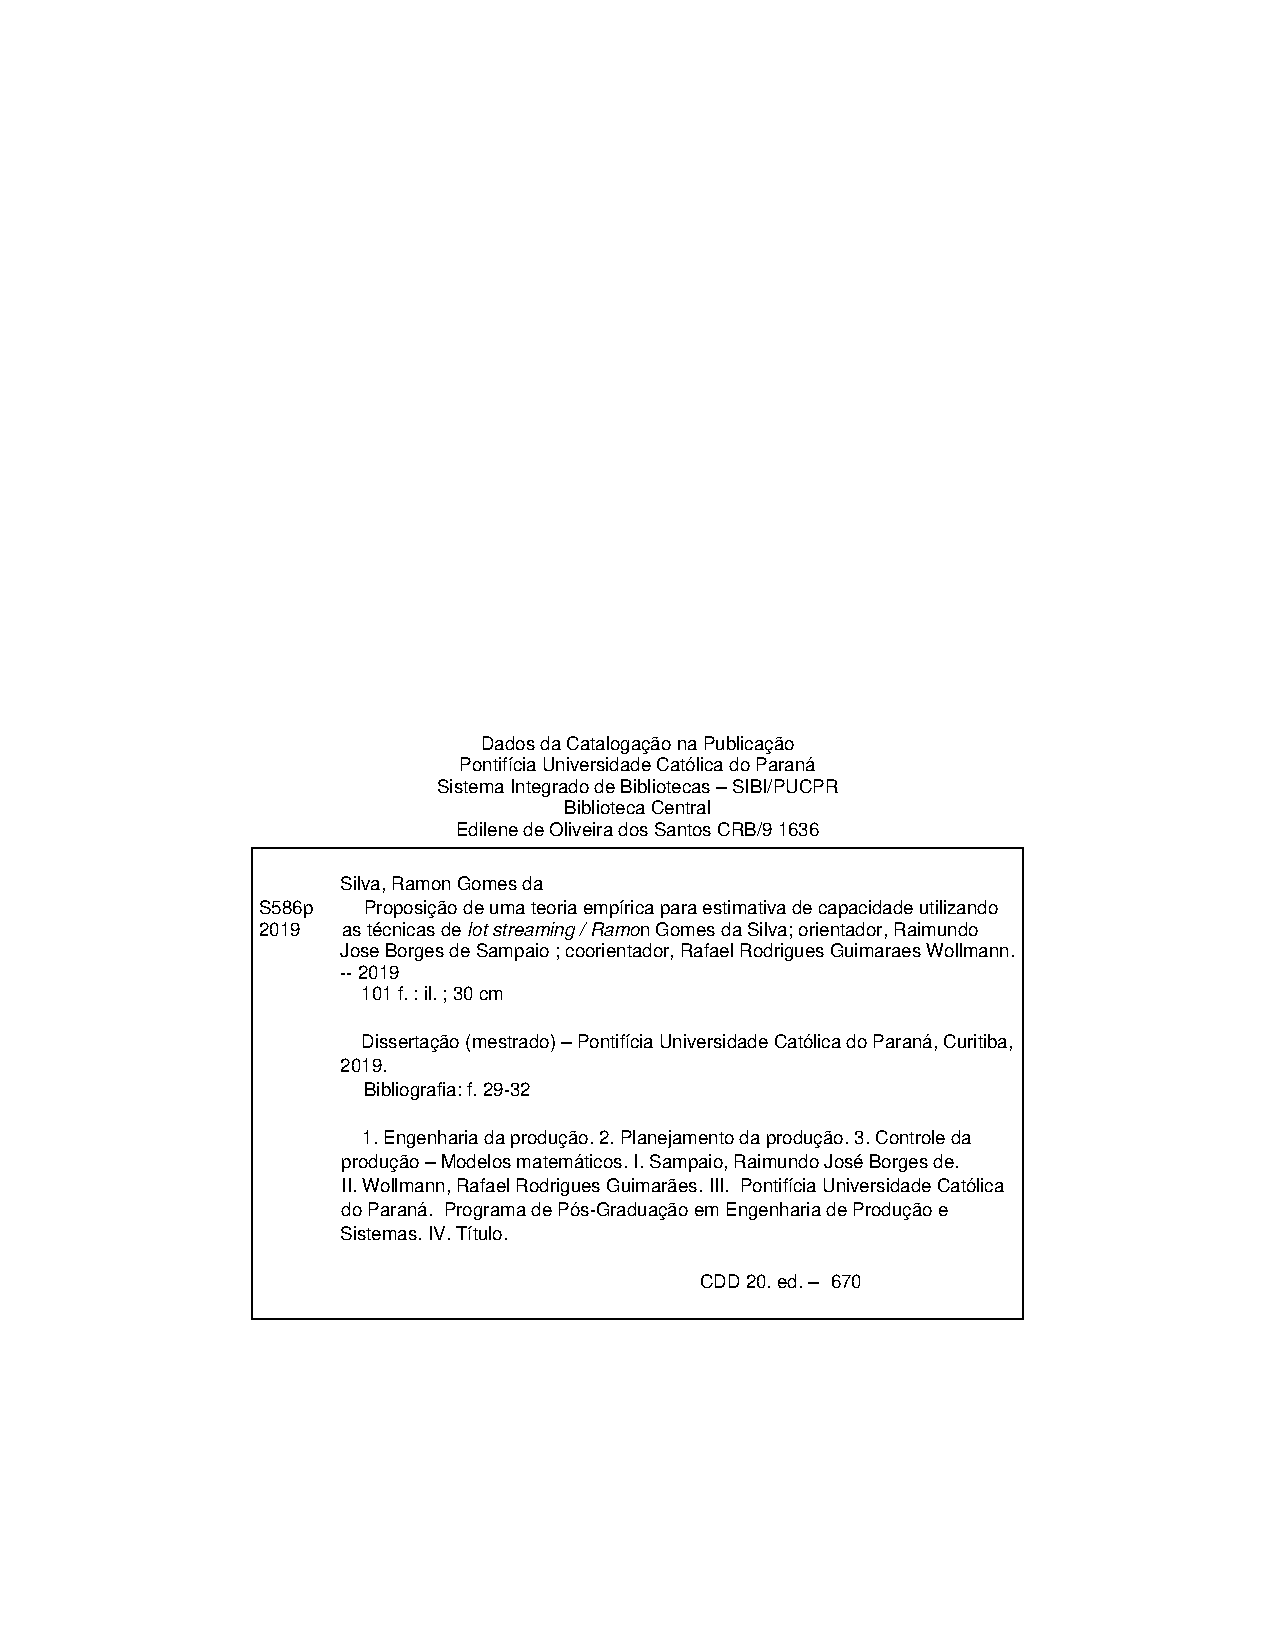
\includepdf{Pretextuais/ficha.pdf}

%% FOLHA DE APROVAÇÃO
%\begin{center}
    {\singlespacing
    \MakeUppercase{\textbf{\aluno}} \\ [1cm]

    \MakeUppercase{\textbf{\titulo}} \\ [1cm]

    \hspace{.45\textwidth} %% POSICIONANDO A MINIPAGE
        \begin{minipage}{.5\textwidth}
        \noindent Dissertação apresentada ao \curso. Área de concentração: Concepção, Logística e Gestão de Sistemas Produtivos, da \departamento, da \universidade, como requisito parcial à obtenção do título de Mestre em Engenharia de Produção e Sistemas. \\ [5mm]
        \end{minipage}
    \textbf{COMISSÃO EXAMINADORA} \\ [1cm]
    
    \rule{10cm}{.1mm} \\ \orientador \\ Orientador\\ \universidade \\ [10mm]

    \rule{10cm}{.1mm} \\ \coorientador \\ Coorientador \\ \universidade \\ [10mm]

    \rule{10cm}{.1mm} \\ \convidadoa \\ Banca \\ \univconvidadoa \\ [10mm]
    
    \rule{10cm}{.1mm} \\ \convidadob \\ Banca \\ \univconvidadob \\ [10mm]
    
    \vfill
    
    \cidade, \datadefesa
    }
\end{center}


%% DEDICATÓRIA
%\vspace*{\fill}
\hspace{.45\textwidth} %% POSICIONANDO A MINIPAGE
    \begin{minipage}{.5\textwidth}
    \flushright
    
    À Deus, à minha família e aos amigos presentes nesse caminhar.
    
    \end{minipage}


%% AGRADECIMENTOS
%\begin{center}
    \textbf{AGRADECIMENTOS}
\end{center}



%% EPÍGRAFE
%\begin{center}
\vspace*{\fill}
\hspace{.45\textwidth} %% POSICIONANDO A MINIPAGE
    \begin{minipage}{.5\textwidth}
    \flushright
    \noindent \textit{``Do \ldots or do not. There is no try''.}
    
    (Mestre Yoda)
    \end{minipage}
\end{center}

%% RESUMO
\begin{abstract}
    \noindent Planejamento e programação da produção são etapas importantes do processo produtivo em um sistema de manufatura. Para garantir que o planejamento e programação de produção de um sistema produtivo sejam satisfatórios é necessário a estimação da capacidade desse sistema da maneira mais precisa. Para garantir essa precisão, são necessárias a utilização de regras de estimação tal como o \textit{lot streaming}, que é uma técnica que subdivide um lote de produção em sublotes menores, para que operações consecutivas possam ser processadas em sobreposição (\textit{overlapping}), isto é, para que possam ser processadas em paralelo. Para problemas gerais, ou seja, sistemas de produção com $m$ máquinas e $n$ sublotes, o problema se torna extremamente complexo. Sistemas de produção desequilibrados geralmente são menos eficientes que sistemas equilibrados. Trabalhar com sistemas desequilibrados e complexos além de caros, necessitam de um conhecimento técnico específico e domínio das técnicas de \textit{lot streaming}, uma vez que não há uma regra geral para problemas com $m$ máquinas e $n$ sublotes. Este trabalho tratou de propor uma teoria empírica que estimasse a capacidade utilizando as técnicas de \textit{lot streaming}, e que fosse uma alternativa mais simples e barata para problemas mais gerais e complexos. Numerosos experimentos numéricos realizados na fase inicial desse estudo sugeriram que sistemas desequilibrados podiam ser representados usando-se sistemas equilibrados equivalentes em certo sentido específico, com um erro que que podia ser estimado a priori. Então planejamos e executamos um experimento numérico para testar a seguinte hipótese: O \textit{makespan} de sistemas de manufatura com $m$ máquinas e $n$ lotes com tempos distintos $p_i$ de processamento em cada máquina $i$ podem ser estimados adequadamente usando-se um tempo médio $p$ para cada máquina? Para responder a essa questão foi planejado e executado um planejamento estatístico do seguinte modo. Os experimentos foram divididos em 9 grupos. Com a utilização do \textit{Software R} foram gerados cenários para cada grupo. São os grupos, sistemas com: 5 máquinas e variação nos tempos de processamentos de até 20\%; 5 máquinas e variação de até 50\%; 5 máquinas e variação de até 70\%; 10 máquinas e variação de até 20\%; 10 máquinas e variação de até 50\%; 10 máquinas e variação de até 70\%; 15 máquinas e variação de até 20\%; 15 máquinas e variação de até 50\%; e, 15 máquinas e variação de até 70\%. Para cada grupo foram gerados 100 cenários com tempos de processamento aleatórios. Para cada um dos cenários aleatórios foi gerado um cenário equilibrado equivalente. Comparando os resultados dos tempos de completude de cada cenário, foi possível observar que sistemas mais equilibrados possuem uma diferença menor que 8\%. O trabalho concluiu que a alternativa oferece resultados mesmo não sendo ótimos, por um custo computacional extremamente baixo. E portanto pode-se construir uma teoria empírica de natureza prática que substitua a difícil tarefa de resolver problemas de \textit{makespan} com $m$ máquinas e $n$ lotes com tempos $p_i$ de processamento de cada máquina. Em conclusão o trabalho apresentado sugere uma teoria empírica para o problema geral de \textit{makespan} com $m$ máquinas e $n$ sublotes com tempos $p_i$ de processamento na máquina $i$ com margem de erro conhecida, usando a teoria disponível para duas e três máquinas, $n$ sublotes, e $p_i$ tempos de processamento de cada máquina $i$. Essa contribuição tem grande relevância prática porque não existe uma solução analítica geral para esse problema de grande interesse dos sistemas de manufatura.   \\ [5mm]
    \textbf{Palavras-chaves:} Capacidade, \textit{Lot Streaming}, Planejamento da Produção, Programação da Produção, Simulação.
\end{abstract}



%% ABSTRACT
{\selectlanguage{english}
\begin{abstract}
    \noindent Production Planning and Scheduling are important phases of the productive process in a manufacturing system. To ensure that the production planning and scheduling of a production system be satisfactory it is necessary the forecast of the capacity as accurate as possible. To ensure this accuracy, it is necessary the utilization of rules of forecast such as the Lot Streaming, which is a technique that divides a production lot into smaller sublots to consecutive operations be processed in overlapping, i.e., it can be processed in parallel. In general problems, i.e., with production systems with $m$ machines and $n$ sublots, the problem becomes extremely complex. Unbalanced production systems are generally less efficient than balanced systems. Working with unbalanced and complex systems, besides being expensive, require a specific technical knowledge and a domain of the lot streaming techniques, once there is no general rule to $m$ machine problems and $n$ sublots. This research worked on propose an empirical theory that estimates capacity using the lot streaming techniques, and that was also a simplest and cheaper alternative to more general and complex problems. Numerous numerical experiments conducted in the early phase of this study suggested that unbalanced systems could be represented using equivalent systems in a certain sense, with an error that could be estimated a priori. So, we planned and executed a numerical experiment to test the following hypothesis: Can the manufacturing systems makespan with $m$ machines and $n$ lots with distinct times $p_i$ of processing in each machine $i$ be estimated properly using a mean time $ p $ for each machine? To answer this question a statistical planning was planned and executed as follows. The experiments were divided in 9 groups. By using R Language, it was generated scenarios for each group. The groups are composed of systems with: 5 machines and variation on process times of 20\%; 5 machines and variation of 50\%; 5 machines and variation of 70\%; 10 machines and variation of 20\%; 10 machines and variation of 50\%; 10 machines and variation of 70\%; 15 machines and variation of 20\%; 15 machines and variation of 50\%; and, 15 machines and variation of 70\%; For each group, 100 scenarios with random process times were generated. For each random scenario it was generated an equivalent balanced scenario. Comparing the results of the completeness times of each scenario, it was possible to observe that more balanced systems have a difference of less than 8\%. The research concluded that the alternative offers results even if not optimal, for an extremely low computational cost. And, therefore, one can construct an empirical theory of practical nature that replaces the difficult task of solving problems of makespan with $m$ machines and $n$ lots with times $p_i$ of processing of each machine. In conclusion the work presented suggests an empirical theory for the general problem of makespan with $m$ machines and $n$ sublots with times $p_i$ of processing in the machine $i$ with known margin of error, using the available theory for two and three machines, $n$ sublots, and $p_i$ processing times of each machine $i$. This contribution has great practical relevance because there is no general analytical solution to this problem of great interest to manufacturing systems. \\ [5mm]
    \noindent \textbf{Keywords:} Capacity, Lot Streaming, Production Planning, Scheduling, Simulation.
\end{abstract}
}


%% LISTA DE TABELAS
%\newpage 
%\pdfbookmark[0]{\listtablename}{lot}
%\listoftables

%% LISTA DE FIGURAS
%\newpage 
%\pdfbookmark[0]{\listfigurename}{lof}
%\listoffigures 

%% LISTA DE ABREVIAÇÕES
%\newpage 
%\printnomenclature

%% SUMÁRIO
\newpage
\pdfbookmark[0]{\contentsname}{toc}
\tableofcontents 

%-----------------------------------------------------------------
%% ELEMENTOS TEXTUAIS

%% INTRODUÇÃO
\include{Introducao/sec:introducao}

%% REFERENCIAL
\include{Referencial/sec:referencial}

%% METODOLOGIA
\include{Metodologia/sec:metodologia}

%% DESCRIÇÃO DO CENÁRIO
\include{Cenario/sec:cenario}

%% RESULTADOS
%\include{Resultados/sec:resultados}

%% CONCLUSÕES
%\include{Conclusoes/sec:conclusoes}

%% CRONOGRAMA
\include{Cronograma/sec:cronograma}

%-----------------------------------------------------------------
%% ELEMENTOS POS-TEXTUAIS

%% BIBLIOGRAFIA
\include{Bibliografia/sec:bibliografia}

\end{document}